\documentclass[norsk,a4paper,12pt]{article}
\usepackage[utf8]{inputenc}
\usepackage{graphicx} %for å inkludere grafikk
\usepackage{verbatim} %for å inkludere filer med tegn LaTeX ikke liker
\usepackage{tabularx}
\usepackage{booktabs}
\usepackage{amsmath}
\usepackage{float}
\usepackage{color}
\usepackage{listings}
\usepackage{hyperref}
\usepackage{amsmath}
\usepackage{empheq}
\usepackage{tikz}
    \usetikzlibrary{positioning}

\definecolor{myblue}{rgb}{.8, .8, 1}

\tikzset{basic/.style={draw,fill=blue!20,text width=1em,text badly centered}}
\tikzset{input/.style={basic,circle}}
\tikzset{weights/.style={basic,rectangle}}
\tikzset{functions/.style={basic,circle,fill=blue!10}}

\lstset{language=Python}
\lstset{basicstyle=\small}
\lstset{backgroundcolor=\color{myblue}}
\lstset{frame=single}
\lstset{stringstyle=\ttfamily}
\lstset{keywordstyle=\color{blue}\bfseries}
\lstset{commentstyle=\itshape\color{blue}}
\lstset{showspaces=false}
\lstset{showstringspaces=false}
\lstset{showtabs=false}
\lstset{breaklines}
\lstset{postbreak=\raisebox{0ex}[0ex][0ex]{\ensuremath{\color{blue}\hookrightarrow\space}}}
\usepackage{titlesec}

\setcounter{secnumdepth}{4}

\titleformat{\paragraph}
{\normalfont\normalsize\bfseries}{\theparagraph}{1em}{}
\titlespacing*{\paragraph}
{0pt}{3.25ex plus 1ex minus .2ex}{1.5ex plus .2ex}

\newlength\mytemplen
\newsavebox\mytempbox

\makeatletter
\newcommand\mybluebox{%
    \@ifnextchar[%]
       {\@mybluebox}%
       {\@mybluebox[0pt]}}

\def\@mybluebox[#1]{%
    \@ifnextchar[%]
       {\@@mybluebox[#1]}%
       {\@@mybluebox[#1][0pt]}}

\def\@@mybluebox[#1][#2]#3{
    \sbox\mytempbox{#3}%
    \mytemplen\ht\mytempbox
    \advance\mytemplen #1\relax
    \ht\mytempbox\mytemplen
    \mytemplen\dp\mytempbox
    \advance\mytemplen #2\relax
    \dp\mytempbox\mytemplen
    \colorbox{myblue}{\hspace{1em}\usebox{\mytempbox}\hspace{1em}}}

\makeatother

\title{A Brief Introduction to Neural Networks\\\vspace{2mm} \Large{1st Edition}}
\author{\large Even Marius Nordhagen}
\date\today
\begin{document}

\maketitle

\begin{itemize}
\item Github repository containing scripts: \url{https://github.com/evenmn/Machine-Learning}
\end{itemize}


\section{Introduction}
This is ment to be a brief theoretical description of single-layer perceptrons and multi-layer perceptrons. In particular I will focus on the concrete theory, but I might add some coding examples as well. 

\subsection{Why do I write this paper?} 
I write this mainly for my own purposes, because it makes it easier to remember all details. Even though there are tons of articles and books about neural networks, I have been struggeling finding a source which describes the the theory in a good way in the same time as it does not get too long. My goal is to give the reader a good understanding in as few lines as possible, such that I can go back and read it myself in case I have forgot something. It might be useful for my master thesis as well. 

I will start with the single perceptron. Thereafter I will move on to the multi-layer perceptron, where backward propagation will be the main focus. Some scripts will hopefully be added, since most (all) of you will use this for numerical purposes.

\subsection{Notation}
The mathematics in this article is NOT complicated, high school maths should be sufficient to understand what is going on. We will use some linear algebra to simplify the expressions and increase the performance of the programs, but it is not a must. Anyway, we are going to deal with a lot of quantities, sometimes with multiple indices, so to follow the calculations it is important that you are familiar with the notation. 
\subsubsection{Quantities}

\subsubsection{Products}
We will apply several kinds of products to get the vectorization right. If you are not familiar with all of them, you should not worry. They are quite simple.

We start with the inner product, or simply the dot product. 
\begin{equation}
\begin{pmatrix}
a_1&a_2&a_3
\end{pmatrix}
\cdot
\begin{pmatrix}
b_1\\b_2\\b_3
\end{pmatrix}
= a_1b_1 + a_2b_2 + a_3b_3.
\end{equation}

Then we have the outer product, which creates a matrix when the vectors are of length 2 or longer. 
\begin{equation}
\begin{pmatrix}
a_1\\a_2\\a_3
\end{pmatrix}
\otimes
\begin{pmatrix}
b_1&b_2&b_3
\end{pmatrix}
= 
\begin{pmatrix}
a_1b_1 & a_1b_2 & a_1b_3\\
a_2b_1 & a_2b_2 & a_2b_3\\
a_3b_1 & a_3b_2 & a_3b_3
\end{pmatrix}
\end{equation}

Last, but not least, we have the Hadamard product (also denoted as the Schul product), which is when we multiply two matrices element wise. It only works when the matrices have the same dimensions, and in our case we will apply it on vectors only. 
\begin{equation}
\begin{pmatrix}
a_1\\a_2\\a_3
\end{pmatrix}
\odot
\begin{pmatrix}
b_1\\b_2\\b_3
\end{pmatrix}
=
\begin{pmatrix}
a_1b_1\\a_2b_2\\a_3b_3
\end{pmatrix}
\end{equation}

\newpage
\section{Single-layer perceptrons}
The principle behind single-layer perceptrons, which is the simplest neural networks, is quite easy to understand. A set of inputs are sent into the network, and a set of outputs is returned. The inputs are multiplied by several weights, and by adjusting those weights a single perceptron can solve every \textit{linear problem} (I come back to this later). A drawing of the single-layer perceptron is found in figure (\ref{fig:single_perceptron}).

\begin{figure} [H]
\centering
\label{fig:single_perceptron}
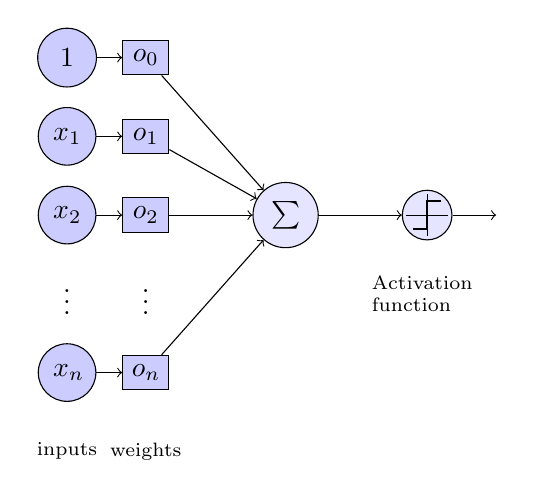
\begin{tikzpicture}
        \node[functions] (center) {};
        \node[below of=center,font=\scriptsize,text width=4em] {Activation function};
        \draw[thick] (0.5em,0.5em) -- (0,0.5em) -- (0,-0.5em) -- (-0.5em,-0.5em);
        \draw (0em,0.75em) -- (0em,-0.75em);
        \draw (0.75em,0em) -- (-0.75em,0em);
        \node[right of=center] (right) {};
            \path[draw,->] (center) -- (right);
        \node[functions,left=3em of center] (left) {$\sum$};
            \path[draw,->] (left) -- (center);
        \node[weights,left=3em of left] (2) {$o_2$} -- (2) node[input,left of=2] (l2) {$x_2$};
            \path[draw,->] (l2) -- (2);
            \path[draw,->] (2) -- (left);
        \node[below of=2] (dots) {$\vdots$} -- (dots) node[left of=dots] (ldots) {$\vdots$};
        \node[weights,below of=dots] (n) {$o_n$} -- (n) node[input,left of=n] (ln) {$x_n$};
            \path[draw,->] (ln) -- (n);
            \path[draw,->] (n) -- (left);
        \node[weights,above of=2] (1) {$o_1$} -- (1) node[input,left of=1] (l1) {$x_1$};
            \path[draw,->] (l1) -- (1);
            \path[draw,->] (1) -- (left);
        \node[weights,above of=1] (0) {$o_0$} -- (0) node[input,left of=0] (l0) {$1$};
            \path[draw,->] (l0) -- (0);
            \path[draw,->] (0) -- (left);
        \node[below of=ln,font=\scriptsize] {inputs};
        \node[below of=n,font=\scriptsize] {weights};
    \end{tikzpicture}
\caption{Single perceptron}
\end{figure}
Initially one needs to train the network such that it knows which outputs are correct, and for that one needs to know the outputs that correspond to the inputs. Every time the network is trained, the weights are adjusted such that the error is smaller. 

The very first step is to calculate the initial outputs, where the weights usually are set to small random numbers. Then the error is calculated, and the weights are updated to minimize the error. So far so good.

\subsection{Getting Outputs}\label{sec:ashortwalkthrough}
Let us look at it from a more mathematically perspective (do not panic, it should not be too complicated), and calculate the netto output. The netto output seen from an output node is simply the sum of all the "arrows" that go to the node, see figure (\ref{fig:single_perceptron}), where each "arrow" is given by the left-hand node multiplied with its respective weight. For example the contribution from input node 2 to output node 1 follows from $X_2\cdot w_{21}$, and the total netto output to $O_1$ is therefore
\begin{equation}
net_1 = \sum_{i=1}^{I} X_i\cdot w_{i1} + b_1\cdot 1.
\end{equation}
Just some notation remarks: $X_i$ is the value of input node $i$ and $w_{ij}$ is the weight which connects input $i$ to output $j$. The parameter $b$ is the bias weight, which we will discuss later. The netto output to a node $j$ is therefore 
\begin{empheq}[box={\mybluebox[5pt]}]{equation}
    net_j = \sum_{i=1}^{I} X_i\cdot w_{ij} + b_j\cdot 1.
\label{eq:forward}
\end{empheq}
You might wonder why we talk about the netto output all the time, do we have other outputs? If we look at the network mathematically, what we talk about as the netto output should be our only output. Anyway, to make the algorithm easy to implement, mapping the netto output to a final output is standard practise. You do not need to care too much about this right now, the mapping is done with a sigmoid function and is explained further in section \ref{sec:sigmoid1}. The sigmoid function takes in the netto output and gives the output, 
\begin{equation}
out_j = \text{sigmoid}(net_j).
\end{equation}
Now all the tools for finding the outputs are in place, and we can calculate the error. If the outputs are larger than the targets (which are the exact answers), the weights need to be reduced, and if the error is large the weights need to be adjusted a lot. The weight adjustment can be done in multiple ways, and we will apply the widely used \textbf{stochastic gradient descent}, which might also be the most basic. The principle is easy: each weight is adjusted with respect to itselfs total error gradient,
\begin{empheq}[box={\mybluebox[5pt]}]{equation}
    w_{ij}^+= w_{ij} - \eta\cdot\frac{\partial E_{TOT}}{\partial w_{ij}},
\label{eq:w_update}
\end{empheq}
where $\eta$ is what we call the learning rate. If not everything is clear right now, it is fine. We will discuss the most important concepts before we dive into the maths.

\subsection{BIAS}
As mentioned above, we use biases when calculating the outputs. The nodes, with value $B$, are called the bias nodes, and the weights, $b$, are called the bias weights. But why do we need those? 

Imagine we have two inputs with value zero, and one output which should not be zero (this could for instance be a NOR gate). Without the bias we will not be able to get any other output than zero, and in fact the network would struggle to find the right weights even if the output had been zero. 

The bias value $B$ does not really matter since the network will adjust the bias weights with respect to it, and is usually set to 1 and ignored in the calculations. The same will be done in this document.

\subsection{Learning rate}
In principle the weights could be updated without adding any learning rate ($\eta=1$), but this can in practise be problematic. It is easy to imagine that the outputs can be fluctuating around the targets without decreasing the error, which is not ideal, and a learning rate can be added to avoid this. The downside is that with a low learning rate the network needs more training to obtain the correct targets (and it takes more time), so we need to find a balance. 

The problem occurs when we are close to the target only, so one solution could be using dynamic learning rate, which decreases when the number of iterations increase,
\begin{equation}
\eta=\frac{\eta_0}{\sqrt{1+\text{iter}}},
\end{equation}
where $\eta_0$ is the initial learning rate and iter is the current iteration. 

Regardless of whether we use dynamic or static learning rate, an usual value is in the interval $(0,0.25]$, but it is not unusual to see values as low as 0.01 (especially for the static case). 


\subsection{Error function}\label{sec:error_function}
The error function we use is inspired by the error function used in \textbf{the least squares method}, and reads
\begin{empheq}[box={\mybluebox[5pt]}]{equation}
    E_{TOT} = \frac{1}{2}\sum_j (y_j - t_j)^2
\label{eq:error_function}
\end{empheq}
where we sum over all the outputs. The factor $1/2$ is added just to give a clean derivative, which in fact makes all the expressions neater. It would also be possible to use other error functions, but to find specific expressions for the weight updating formulae, we better focus on the one above. 

\subsection{Sigmoid function}\label{sec:sigmoid1}
Inspired by Boolian algebra, the inputs and outputs initially are set to either 0, 1, or a superposition of them. To ensure that every output is between 0 and 1, we map them all using a sigmoid function. Perhaps the most common function to use is
\begin{empheq}[box={\mybluebox[5pt]}]{equation}
    f(x)=\frac{1}{1+\exp(-x)}
\label{eq:sigmoid}
\end{empheq}
which maps between 0 and 1 as required. Another important property is that the derivative of this function has a quite easy form, which is important. The derivative of this function is
\begin{equation}
f'(x)=f(1-f)
\end{equation}
and the derivation of it is shown carefully in Appendix A. The function is presented in figure (\ref{fig:sigmoid1}).
\begin{figure} [H]
    \centering
    \includegraphics[scale=0.65]{images/sigmoid1.png}
    \caption{A sigmoid function plotted from -8 to 8. The asymphtotes are drawn to stress that the function will approach the value 1 when $x\rightarrow \infty$ and the value 0 when $x\rightarrow -\infty$.}
    \label{fig:sigmoid1}
\end{figure} 

We can also use other sigmoid functions which not even map between 0 and 1, for instance another well-known sigmoid function reads
\begin{empheq}[box={\mybluebox[5pt]}]{equation}
    f(x)=\tanh(x)=\frac{\exp(x)-\exp(-x)}{\exp(x) + \exp(-x)}
\end{empheq}
which maps between -1 and 1. Apart from that, the function looks quite similar to the sigmoid function in equation (\ref{fig:sigmoid1})\\
\begin{figure} [H]
    \centering
    \includegraphics[scale=0.65]{images/sigmoid2.png}
    \caption{A sigmoid function plotted from -8 to 8. The asymphtotes are drawn to stress that the function will approach the value 1 when $x\rightarrow \infty$ and the value -1 when $x\rightarrow -\infty$.}
    \label{fig:sigmoid2}
\end{figure} 
Also this function got a simple derivative, given by
\begin{equation}
\frac{d\tanh(x)}{dx}=\frac{1}{\cosh^2(x)}=\frac{4}{(\exp(x)+\exp(-x))^2}
\end{equation}
which is shown in Appendix B. 

\subsection{Update weights}
Now we have the fundamentals to go further with the theory expressed in section \ref{sec:ashortwalkthrough}. Actually, the only thing we are left with is finding an expression for the weight updating based on the formula from equation (\ref{eq:w_update}), 
\begin{equation}
w_{ij}^+= w_{ij} - \eta\cdot\frac{\partial E_{TOT}}{\partial w_{ij}},
\end{equation}
where the partial derivative is what we need to find. Since the energy is not directly dependent on $w_{ij}$, we need to do a change of variables such that we get derivatives we can calculate. Probably the best choice is
\begin{equation}
\frac{\partial E_{TOT}}{\partial w_{ij}}=\frac{\partial E_{TOT}}{\partial out_{j}}\cdot\frac{\partial out_{j}}{\partial net_{j}}\cdot\frac{\partial net_{j}}{\partial w_{ij}}.
\end{equation}
Standard differentiating of the error function from section \ref{sec:error_function} gives
\begin{equation}
\frac{\partial E_{TOT}}{\partial out_{j}}=-(t_j-out_j)
\end{equation}
which is a neat expression as pointed out above. To obtain the second fraction, we need to decide which sigmoid function to use. In the calculations I will use the first mentioned in section \ref{sec:sigmoid1}, that reads
\begin{equation}
out_j=\frac{1}{1+\exp(-net_j)}.
\end{equation}
and we have already found that
\begin{equation}
\frac{\partial out_{j}}{\partial net_{j}}=out_j(1-out_j).
\end{equation}
Furthermore the netto output is given by equation (\ref{eq:forward}),
\begin{equation}
net_j = \sum_{i=1}^{I} X_i\cdot w_{ij} + b_j\cdot 1,
\end{equation}
which simply gives
\begin{equation}
\frac{\partial net_{j}}{\partial w_{ij}}=X_i.
\end{equation}
We end up with 
\begin{equation}
\frac{\partial E_{TOT}}{\partial w_{ij}}=-(t_j-out_j)\cdot out_j(1-out_j)\cdot X_i
\end{equation}
and the weight updating formula
\begin{empheq}[box={\mybluebox[5pt]}]{equation}
    w_{ij}^{+}=w_{ij} + \eta\cdot(t_j-out_j)\cdot out_j(1-out_j)\cdot X_i
\end{empheq}
Similarly we need to update the bias weights, with a formula similar to that one in equation (\ref{eq:w_update}):
\begin{equation}
b_i^+=b_i - \eta\cdot\frac{\partial E_{TOT}}{\partial b_i}.
\end{equation}
We do the same change of variables and the only thing that changes is the last part, $\partial net_i/\partial b_i$, which can easily be found to be 1. Then
\begin{empheq}[box={\mybluebox[5pt]}]{equation}
    b_i^+=b_i + \eta\cdot(t_i-out_i)\cdot out_i(1-out_i)
\end{empheq}
and all the basics for the single perceptron are set. 

\subsection{Algorithm}
The actual algorithm consists of the results above, and we need to order them correctly. To increase the performance and the neatness, I will present a vectorized implementation (i.e. use linear algebra to solve it instead of sum over piecewise elements). For the forward propagation (when we get the outputs), it is easy to see that it can be vectorized,
\begin{equation}
net_j = \sum_i (w_{ij}\cdot X_i + b_i)\quad\Rightarrow\quad net = W\cdot X + b.
\end{equation}
where $net$ is a vector. Also the backward propagation (when we update the weights) can be vectorized. Firstly the differentiation of the error function can be vectorized:
\begin{equation}
\frac{\partial E_{TOT}}{\partial out_i}=-(t_i-out_i)\quad\Rightarrow\quad \frac{\partial E_{TOT}}{\partial out}=-(t-out)
\end{equation}
where we have vectors on both sides. Those vectors will have the same length as $out(1-out)$, such that we can define a quantity $\delta^o$ and apply the Hadamard multiplication:
\begin{equation}
\delta^o = \frac{\partial E_{TOT}}{\partial out}\odot\frac{\partial\text{sigmoid}(out)}{\partial out}=-(t-out)\odot out(1-out)
\end{equation}
which will be used in both the weight update and the bias update. To fulfil the weight update, we need to take the outer product of $\delta^o$ with the inputs $X_i$, and we then have $\partial E_{TOT}/\partial W$, which of course has the same dimensions as the weight matrix. 
\begin{equation}
W^+ = W - \eta(\delta^o\otimes X)
\end{equation}
\begin{equation}
b^+ = b - \eta\cdot\delta^o
\end{equation}

It should look something like this:
\begin{itemize}
\item \textbf{Declare all variables, define inputs, targets and quantities, and initialize the weights}\\
\#Iterations = ...\\
Eta = ...\\
\\
X = [[...] ... [...]]\\
t = [[...] ... [...]]\\
\\
W = 2*random(0,1) - 1\\
b = 2*random(0,1) - 1\\

\item \textbf{Training - calculate outputs for all samples and then update weights. Repeat \#Iterations times}\\
for i < \#Iterations\\
	for j < \#Samples\\
		net = X*W + b\\
		out = sigmoid(net)\\
		\\
		W = W + eta*(t - out)*out(1-out)*X\\
		b = b + eta*(t - out)*out(1-out)\\

\item \textbf{Recall - Use the weight to find answer to problems with unknown answers}\\
X = [[...] ... [...]]		Inputs with unknown outputs\\
net = X*W + b\\
ans = sigmoid(out)\\
\end{itemize}

\subsection{Implementation}
For simplicity all the example codes will be Python scripts, and the numpy package will be used diligently because of its linear algebra features and its performance. Similarly one can use armadillo in C++ and if you wonder how to do the implementations in there, you could visit my github repository. Anyway, the best way to implement the algorithm is with a function which takes the parameters as arguments and returns the weights. We define all quantities as numpy arrays, and use \lstinline!np.dot! for the inner product, \lstinline!np.outer! for the outer product and simply multiply two arrays for the Hadamard product. If you do not trust this latter statement, \lstinline!np.multiply! should be corresponding. The implementation looks like this;

\lstset{basicstyle=\scriptsize}
\begin{lstlisting}
def linear(X, t, T, eta = 0.1):
    
    I = len(X[0])
    O = len(t[0])
    M = len(X)
    
    W = 2*np.random.random([I, O]) - 1
    b = 2*np.random.random(O) - 1

    for iter in range(T):
        for i in range(M):
            net = np.dot(X[i], W) + b
            out = sigmoid(net)

            deltao = -(t[i] - out)*sig_der(out)
            W = W - eta * np.outer(np.transpose(X[i]), deltao)
            b = b - eta * deltao
    return W, b
    
\end{lstlisting}
where sigmoid is the sigmoid function used in the weight calculations above and sig\_der is its derivative. To get this working, the input array $X$ and the target array $t$ need to be numpy arrays, and a call to the function can be done like this
\begin{lstlisting}
X = np.array([[0,0], [0,1], [1,0], [1,1]])
t = np.array([[0], [1], [1], [1]])

W, b = linear(X, t, 1000)
\end{lstlisting}
which can be recognized as an OR gate. The logic functions are popular examples when it comes to neural network, because (1) they are easy to work with (2) they display the constraints of a single perceptron in a easy way. In next section we are going to discuss this, and why we need multi-layer perceptrons for certain logic functions. However, back to the implementation. Since we now know the weights, we can use them to recall, which is simply done by
\begin{lstlisting}
X_ = np.array([0,1])
net = np.dot(X_, W) + b
out = sigmoid(net)
print(out)
>>> 1
\end{lstlisting}
which should give 1 according to the OR gate. We could train this network to understand NOR, AND and NAND gates as well, but what happens if you try to teach it the XOR gate? 

For complete programs, please visit \\ \url{https://github.com/evenmn/Machine-Learning}.

\subsection{Constraints}
It is naturally that such a simple algorithm has constraints, and in fact it is only able to solve so-called linear problems. The logic functions, such as OR, NOR, AND and NAND are common examples, which all can be implemented using a single perceptron. Let us take a closer look at the OR gate.

You might remember the OR gate, but in case you do not, I will refresh the theory. As long as at least one of the inputs are 1, the OR gate will return 1. In a coordinate system it can be drawn as\\
INSERT TABLE HERE\\
For this example we can distinguish the ones from the zero with one single straight line, making it a linear problem (see Figure ()). If we, on the other hand, study the XOR gave which returns 1 when exactly one of the inputs are 1, we no longer have a linear problem, and need to add more layers (again, see figure ()). \\
INSERT PICTURE\\

In fact, every problem can be solved by a two-layer perceptron, according to \textbf{the universal approximation theorem}. However, in many cases we do not know how many nodes that are sufficient, and it might be just as smart to add another layer to ensure that you have enough weights. 

\newpage
\section{Multi-layer Perceptrons}
Start with 2-layer neural network\\
\begin{figure}[H]
\centering
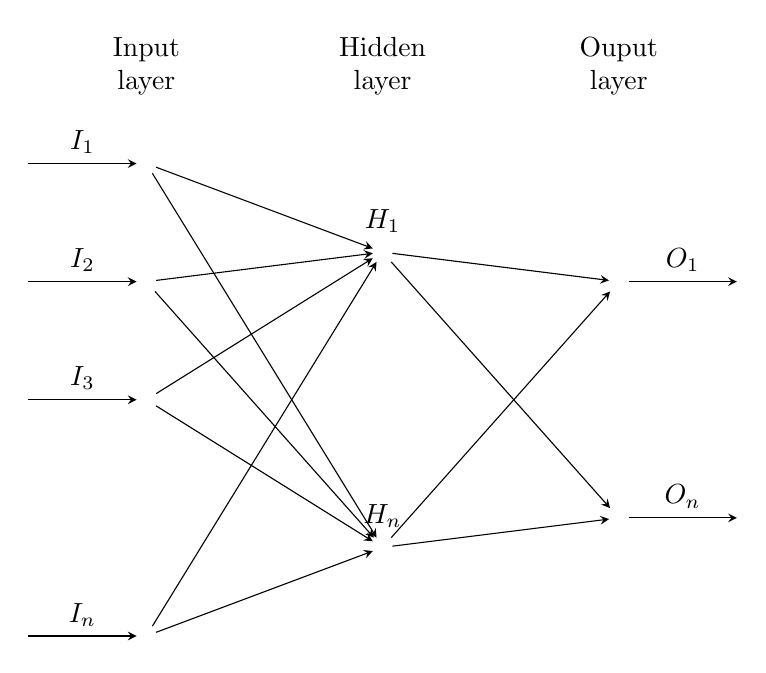
\begin{tikzpicture}[x=1.5cm, y=1.5cm, >=stealth]

\foreach \m/\l [count=\y] in {1,2,3,missing,4}
  \node [every neuron/.try, neuron \m/.try] (input-\m) at (0,2.5-\y) {};

\foreach \m [count=\y] in {1,missing,2}
  \node [every neuron/.try, neuron \m/.try ] (hidden-\m) at (2,2-\y*1.25) {};

\foreach \m [count=\y] in {1,missing,2}
  \node [every neuron/.try, neuron \m/.try ] (output-\m) at (4,1.5-\y) {};

\foreach \l [count=\i] in {1,2,3,n}
  \draw [<-] (input-\i) -- ++(-1,0)
    node [above, midway] {$I_\l$};

\foreach \l [count=\i] in {1,n}
  \node [above] at (hidden-\i.north) {$H_\l$};

\foreach \l [count=\i] in {1,n}
  \draw [->] (output-\i) -- ++(1,0)
    node [above, midway] {$O_\l$};

\foreach \i in {1,...,4}
  \foreach \j in {1,...,2}
    \draw [->] (input-\i) -- (hidden-\j);

\foreach \i in {1,...,2}
  \foreach \j in {1,...,2}
    \draw [->] (hidden-\i) -- (output-\j);

\foreach \l [count=\x from 0] in {Input, Hidden, Ouput}
  \node [align=center, above] at (\x*2,2) {\l \\ layer};

\end{tikzpicture}
\caption{...}
\end{figure}

For the single perceptron the updating of weights was quite straight forward, but for a perceptron consisting of multiple layers the question is: how do we update the weights when we do not know the value of the hidden nodes. And how do we know which layer that causes the error? This will be explained in the next subsection, where one of the most popular techniques for this is taken into account.

\subsection{Forward Propagation}

\subsection{Backward Propagation}
Backward propagation is probably the most used technique to update the weights, and is actually based on equation (\ref{eq:w_update}), but we neglect the $x_i$:
\begin{equation}
w_{ij}^{\dagger}=w_{ij} - \eta\cdot \frac{\partial E_{TOT}}{\partial w_{ij}}.
\end{equation}
To work the partial derivative out, we need to do a change of variables. I will focus on a 2-layer network, but the principle is the same for networks of more layers. The method will be slightly different for the two set of weights (W1 and W2), so I will do it seperately for them. We start with W2, which is naturally since we move backwards (hence backward propagation). 
\begin{align}
\frac{\partial E_{TOT}}{\partial w_{ij}}&=\frac{\partial E_{TOT}}{\partial out_{oj}}\cdot\frac{\partial out_{oj}}{\partial net_{oj}}\cdot\frac{\partial net_{oj}}{\partial w_{ij}}\\
&=\delta_{oj}\cdot\frac{\partial net_{oj}}{\partial w_{ij}}
\end{align}
where $\delta_{oj}$ is the same for all weights that go to the same output $oj$ $\Rightarrow$ we will have $O$ different $\delta_{oj}$'s. Further recall the error function from equation (\ref{eq:error_function}), and recognize that
\begin{equation}
\frac{\partial E_{TOT}}{\partial out_{oj}}=-(t_{oj}-out_{oj})
\end{equation}
where $t_{oj}$ are the targets. Then we have the sigmoid function where we get $out_{oj}$ when we send in $net_{oj}$:
\begin{equation}
out_{oj}=\frac{1}{1+\exp(-net_{oj})}
\end{equation}
such that
\begin{equation}
\frac{\partial out_{oj}}{\partial net_{oj}}=out_{oj}(1-out_{oj})
\end{equation}
as mentioned in section 1 and proven in Appendix A. We end up with
\begin{equation}
\delta_{oj}=-(t_{oj}-out_{oj})\cdot out_{oj}(1-out_{oj})=\frac{\partial E_{TOT}}{\partial net_{oj}}.
\end{equation}
We also have that
\begin{equation}
net_{oj}=\sum_k w_{kj}\cdot out_{hk} + b_{2j}\cdot 1
\end{equation}
such that
\begin{equation}
\frac{\partial net_{oj}}{\partial w_{ij}}=out_{hi}
\end{equation}
and 
\begin{equation}
\frac{\partial E_{TOT}}{\partial w_{ij}}=\delta_{oj}\cdot out_{hi}.
\end{equation}
The specific updating algorithm is the following
\begin{empheq}[box={\mybluebox[5pt]}]{equation}
    w_{ij}^{(2)}\rightarrow w_{ij}^{(2)} - \eta\cdot\delta_{oj}\cdot out_{hi}
\end{empheq}
with 
\begin{equation*}
\delta_{oj}=-(t_{oj}-out_{oj})\cdot out_{oj}(1-out_{oj})
\end{equation*}
We are now set for updating the last weights W2, see section \ref{sec:multi_algorithm} for a overview of the algorithm, section \ref{sec:vectorization} for a short description of how to vectorize the algorithm, or if you want to go straight to the implementation, you should check out section \ref{sec:multi_implementation}. 

However, we also need to update the remaining weights, W1, what are we waiting for? The approach is the same as above with considering how much the total error will change when changing one of the weights and doing a change of variables
\begin{equation}
\frac{\partial E_{TOT}}{\partial w_{ij}}=\frac{\partial E_{TOT}}{\partial out_{hj}}\cdot\frac{\partial out_{hj}}{\partial net_{hj}}\cdot\frac{\partial net_{hj}}{\partial w_{ij}}.
\end{equation}
A difference is that the error for each of the hidden nodes is dependent on the error at each output nodes, such that now $E_{TOT}$ needs to be split up in $O$ terms
\begin{equation}
E_{TOT}=E_{o1} + E_{o2} + \hdots + E_{oO}.
\end{equation}
This causes
\begin{equation}
\frac{\partial E_{TOT}}{\partial out_{hj}}=\frac{\partial E_{o1}}{\partial out_{hj}} + \frac{\partial E_{o2}}{\partial out_{hj}} + \hdots + \frac{\partial E_{oO}}{\partial out_{hj}}
\end{equation}
where we again need to do a change of variables on each of those
\begin{equation}
\frac{\partial E_{ok}}{\partial out_{hj}}=\frac{\partial E_{ok}}{\partial net_{ok}}\cdot\frac{\partial net_{ok}}{\partial out_{hj}}.
\end{equation}
We could have done another change of variables above to avoid equation (\ref{eq:dEokdnetoj}), but this is neater
\begin{equation}
\frac{\partial E_{ok}}{\partial net_{ok}}=\frac{\partial E_{ok}}{\partial out_{ok}}\cdot \frac{\partial out_{ok}}{\partial net_{ok}}.
\label{eq:dEokdnetoj}
\end{equation}
Now it gets more similar to the first weight updates again:
\begin{equation}
\frac{\partial E_{ok}}{\partial out_{ok}}=-(t_{ok}-out_{ok})
\end{equation}
and
\begin{equation}
\frac{\partial out_{ok}}{\partial net_{ok}} = out_{ok}(1-out_{ok}).
\end{equation}
Further we need to calculate $\partial net_{ok}/\partial out_{hj}$, which is done by
\begin{equation}
net_{ok} = \sum_i w_{ik}^{(2)}\cdot out_{hi} + b_{2k}\cdot 1
\end{equation}
and
\begin{equation}
\frac{\partial net_{ok}}{\partial out_{hj}}=w_{jk}^{(2)}
\end{equation}
and we end up with
\begin{equation}
\frac{\partial E_{ok}}{\partial out_{hj}}=-(t_{ok}-out_{ok})\cdot out_{ok}(1-out_{ok})\cdot w_{jk}^{(2)}.
\end{equation}
That was the difficult part, as we have seen before
\begin{equation}
\frac{\partial out_{hj}}{\partial net_{hj}}=out_{hj}(1-out_{hj})
\end{equation}
and since
\begin{equation}
net_{hj} = \sum_l w_{lj}\cdot x_l
\end{equation}
where $x_i$ is input $i$, we obtain
\begin{equation}
\frac{\partial net_{hj}}{\partial w_{ij}}=x_i
\end{equation}
and we finally end up with 
\begin{equation}
\frac{\partial E_{TOT}}{\partial w_{ij}^{(1)}}=\sum_{k=1}^{O}-(t_{ok}-out_{ok})\cdot out_{ok}(1-out_{ok})\cdot w_{jk}^{(2)}\cdot out_{hj}(1-out_{hj})\cdot x_i.
\end{equation}
We recognize the first part as $\delta_{ok}$, such that
\begin{empheq}[box={\mybluebox[5pt]}]{equation}
    w_{ij}^{(1)}\rightarrow w_{ij}^{(1)} - \eta\cdot\sum_{k=1}^{O}\delta_{ok}\cdot w_{jk}^{(2)}\cdot out_{hj}(1-out_{hj})\cdot x_i
\end{empheq}
where we recall $\delta_{ok}$ as
\begin{equation*}
\delta_{ok}=-(t_{ok}-out_{ok})\cdot out_{ok}(1-out_{ok}).
\end{equation*}

Additionally we need to update the bias weights for every iteration, and this can be done in a similar way. Inspired by the standard weight update formula from equation (\ref{eq:w_update}), 

\subsection{Algorithm}\label{sec:multi_algorithm}
This is just a revision of the teory above

\subsection{Vectorization}\label{sec:vectorization}
In the next section we will look at how the implementation goes, but before that it is convenient to look at how we can vectorize the expressions to avoid loops and other time consuming stuff. In the same way as for the single-layer perceptron, we can vectorize the forward propagation as follows
\begin{equation}
net_{hj} = \sum_i (w_{ij}^{(1)}\cdot X_i + b_i^1)\quad\Rightarrow\quad net_h = W_1\cdot X + b^1
\end{equation}
and similar for the netto out vector
\begin{equation}
net_{oj} = \sum_i (w_{ij}^{(2)}\cdot out_{hi} + b_i^2)\quad\Rightarrow\quad net_o = W_2\cdot out_h + b^2.
\end{equation}

The updating algorithm for $W_1$ is done in the same way as we did for the single perceptron, but instead of taking the outer product with $X_i$, we need to do it with $out_h$. 
\begin{equation}
W^+ = W - \eta(\delta^o\otimes out_h)
\end{equation}
\begin{equation}
b^+ = b - \eta\cdot\delta^o
\end{equation}
where $\delta^o$ still focus on the last output. To update the first weight matrix, $W_1$, we first want to get rid of the sum, which can be recognized as the inner product between $\delta^o$ and row $j$ of the matrix $W_2$:
\begin{equation}
\sum_{k=1}^{O}\delta_{k}^o\cdot w_{jk}^{(2)}=\delta_1^ow_{j1}^{(2)}+\delta_2^ow_{j2}^{(2)}+\delta_3^ow_{j3}^{(2)}+\hdots=\delta^ow_{j:}^{(2)}
\end{equation}


\subsection{Implementation}\label{sec:multi_implementation}
\begin{lstlisting}
h
\end{lstlisting}

\subsection{Networks of more layers}
Now as we know how to treat networks with a hidden layer, we can go on adding another layer. Again, the difficult part is the backward propagation, which gonna be ever more messy when we increase the number of layers. Anyway, the principle is the same where we start with the general weight update formula known from \textbf{Gradient Descent}, and do the same change of variables. The hope is that we can recognize a  pattern after calculating the updating formulas for a 3-layer network. \\
ADD FIGURE\\
Since it will be quite a lot calculations, I will just express the results here, and move the calculations to Appendix C. Let us start with the forward propagation:
\begin{empheq}[box={\mybluebox[5pt]}]{align}
net_{hi}&=\sum_jw_{ji}^{(1)}\cdot i_j + b_{1i}\cdot 1\notag\\
out_{hi}&=\text{sig}(net_{hi})\notag\\
\notag\\
net_{ki}&=\sum_jw_{ji}^{(2)}\cdot out_{hj} + b_{2i}\cdot 1\\
out_{ki}&=\text{sig}(net_{ki})\notag\\
\notag\\
net_{oi}&=\sum_jw_{ji}^{(3)}\cdot out_{kj} + b_{3i}\cdot 1\notag\\
out_{oi}&=\text{sig}(net_{oi})\notag
\end{empheq}
which can easily be turned into vector form. The backward propagation follows from the 2-layer example, and we get
\begin{empheq}[box={\mybluebox[5pt]}]{align}
w_{ij}^{(3)}&=w_{ij}^{(3)}-\eta\cdot\delta_{oj}\cdot out_{ki}\notag\\
\notag\\
w_{ij}^{(2)}&=w_{ij}^{(2)}-\eta\sum_{k=1}^O\delta_{ok}\cdot w_{jk}^{(3)}\cdot out_{kj}(1-out_{kj})\cdot out_{hi}\notag\\
\notag\\
w_{ij}^{(1)}&=w_{ij}^{(1)}-\eta\sum_{k=1}^O\sum_{l=1}^K\delta_{ok}\cdot w_{lk}^{(3)}\cdot out_{kl}(1-out_{kl})\cdot w_{jl}^{(2)}out_{hj}(1-out_{hj})\cdot x_i\notag
\end{empheq}
where we again use the short hand 
\begin{equation*}
\delta_{oj}=(t_j-out_{oj})\cdot out_{oj}(1-out_{oj}).
\end{equation*}
If we compare with the weight update formulae for the 2-layer case, we can see some obvious connections, and it is easy to imagine that one can contruct a general weight update algorithm which fits no matter how many layers we have. 

\section{References}
MARSLAND

\newpage
\section{Appendices}
\subsection{Appendix A}
If we differentiate the sigmoid function 
\begin{equation}
f(x)=\frac{1}{1+\exp(-x)}
\end{equation}
from equation (\ref{eq:sigmoid}), and we will get
\begin{equation}
f'(x)=f(1-f)
\end{equation}

\textbf{PROOF:}
\begin{align*}
f'(x) &= -1\cdot(1+\exp(-x))^{-2}\cdot -1\cdot\exp(-x)\\
&=\frac{\exp(-x)}{(1+\exp(-x))^{2}}\\
&=\frac{1+\exp(-x)-1}{(1+\exp(-x))^{2}}\\
&=\frac{1+\exp(-x)}{(1+\exp(-x))^{2}} - \frac{1}{(1+\exp(-x))^{2}}\\
&=\frac{1}{1+\exp(-x)} - \frac{1}{(1+\exp(-x))^{2}}\\
&=\frac{1}{1+\exp(-x)}\bigg(1 - \frac{1}{1+\exp(-x)}\bigg)\\
&=f(1-f)
\end{align*}

\subsection{Appendix B}
We got that
\begin{equation}
\tanh(x)=\frac{e^x-e^{-x}}{e^x + e^{-x}}
\end{equation}
and I stated that
\begin{equation}
\frac{d\tanh(x)}{dx}=\frac{1}{\cosh^2(x)}=\frac{4}{(e^x+e^{-x})^2}.
\end{equation}
We are now gonna prove that:
\begin{align*}
\tanh'(x)&=\frac{e^x + e^{-x}}{e^x + e^{-x}} + (e^{x} - e^{-x})\cdot-1(e^x + e^{-x})^{-2}\cdot(e^x - e^{-x})\\
&=1-\frac{(e^x - e^{-x})^2}{(e^x + e^{-x})^2}\\
&=1-\tanh^2(x)\\
&=\frac{\cosh^2(x)}{\cosh^2(x)}-\frac{\sinh^2(x)}{\cosh^2(x)}\\
&=\frac{1}{\cosh^2(x)}\\
&=\frac{4}{(e^x+e^{-x})^2}
\end{align*}
where we have used that $2\cosh(x)\equiv e^x + e^{-x}$, $2\sinh(x)\equiv e^x - e^{-x}$ and the relation
\begin{align*}
\cosh^2(x)-\sinh^2(x) &= \frac{1}{4}(2\cdot e^x\cdot e^{-x} + 2\cdot e^x\cdot e^{-x})\\
&=\frac{e^x}{e^x}=1
\end{align*}
\end{document}
